\documentclass[aspectratio=169]{beamer}
\usetheme{hogent}
\usecolortheme{hgwhite} % witte achtergrond, zwarte tekst

%% common.tex -- Code die in elk .tex-bestand terug komt

%% Packages

\usepackage[dutch]{babel}
\usepackage{graphicx}
\usepackage{comment,enumerate,hyperref}
\usepackage{amsmath,amsfonts,amssymb}
\usepackage{eurosym}
\usepackage{booktabs}
\usepackage{multicol,multirow}
\usepackage{listings}

\usepackage[outputdir=out]{minted}
%\usepackage{minted}

\usepackage[backend=biber,style=apa]{biblatex}
\DeclareLanguageMapping{dutch}{dutch-apa}

\usepackage{csquotes}

%% Variabelen, elk academiejaar aan te passen
\newcommand{\academicyear}{2023--2024 (revisie: \today)}
\newcommand{\lecturers}{Thomas Aelbrecht \and Thomas Parmentier \and Bert Van Vreckem}
\newcommand{\coursename}{Research Methods (IT)}

%% Macro's en commando's

%% \alertbox: een kader voor tekst die moet opvallen
\newcommand{\alertbox}[2][hgblue]{%
  \setbeamercolor{alertbox}{bg=#1,fg=white}
  \begin{beamercolorbox}[sep=2pt,center]{alertbox}
    \textbf{#2}
  \end{beamercolorbox}
}


%---------- Info over de presentatie ------------------------------------------

\title{Module 6. Rapporteren over onderzoek in \LaTeX{}.}
\subtitle{Research Methods}
\author{\lecturers}   % Pas waarden aan in common.tex
\date{\academicyear}

\begin{document}

\begin{frame}
  \maketitle
\end{frame}

\begin{frame}
  \frametitle{Inhoud}

  \tableofcontents
\end{frame}

\section{Controle installatie}

\begin{frame}
  \frametitle{Heeft iedereen een werkende {\LaTeX}-installatie?}

  \begin{itemize}
    \item Compileert paper tot PDF?
    \item Is bibliografie zichtbaar? (F5-F8-F5)
    \item Correcte referenties in de tekst?
    \item Errors tijdens compilatie?
    \item Fouten in de PDF?
  \end{itemize}

\end{frame}

\section{Korte tips}


\begin{frame}
  \frametitle{Controle installatie, compiler}

  \begin{itemize}
    \item Mik{\TeX} Console: controle op updates
          \begin{itemize}
            \item Als Administrator
            \item Als gewone gebruiker
          \end{itemize}
    \item Instellingen TeXstudio
          \begin{itemize}
            \item Compiler (\texttt{xelatex})
            \item Bibliografie (\texttt{biber}/\texttt{biblatex})
          \end{itemize}
  \end{itemize}

\end{frame}

\begin{frame}
  \frametitle{Controle bibliografie}

  \begin{itemize}
    \item Is de bibliografie niet aanwezig?
          \begin{itemize}
            \item F5 - F8 - F5
            \item of: Tools > Build - Bibliography - Build
          \end{itemize}
    \item Zie je dit soort referenties in de tekst? (\textbf{Doe2021})
          \begin{itemize}
            \item m.a.w.~Bib{\TeX}-key in het vet
            \item Zorg dat bibliografie gecompileerd is
            \item Controleer Bib{\TeX}-key (output van biber)
            \item Na hercompileren zie je (Doe, 2021)
          \end{itemize}
  \end{itemize}

\end{frame}

\begin{frame}[fragile]
  \frametitle{Correct gebruik van aanhalingstekens}

  \textcolor{red}{\textbf{FOUT:}} \verb|"Een tekst"| $\Rightarrow$ \"Een tekst"

  \bigskip

  \textcolor{green}{\textbf{JUIST:}} \verb|``Een tekst''| $\Rightarrow$ ``Een tekst''

  \bigskip

  Gebruik twee ``backquotes'' (links) of twee enkele aanhalingstekens (rechts)
\end{frame}

\begin{frame}
  \frametitle{Welk commando voor dit symbool?}

  \url{https://detexify.kirelabs.org/classify.html}

  \centering
  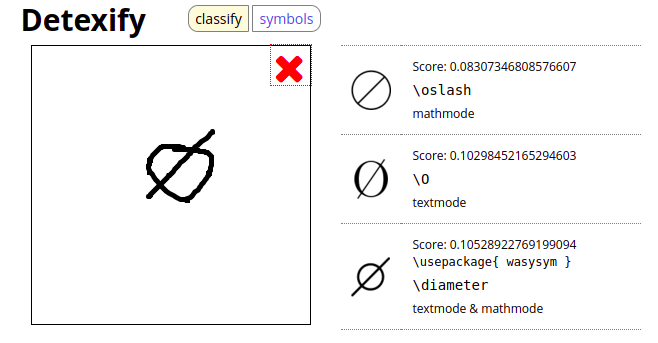
\includegraphics[height=.6\textheight]{6/detexify}

\end{frame}

\begin{frame}[fragile]
  \frametitle{URLs invoegen}

  \begin{itemize}
    \item Via package \texttt{hyperref} (al geladen in sjablonen!)
    \item Commando \verb+\url{}+, \verb+\href{}{}+
    \item Hyperref zorgt ook voor:
          \begin{itemize}
            \item Inhoudstafel in de PDF
            \item Aanklikbare verwijzingen binnen document
          \end{itemize}
  \end{itemize}

\end{frame}

\begin{frame}[fragile]
  \frametitle{URLs invoegen: voorbeeld}

  \verb+\url{https://xkcd.com/1301/}+ $\Rightarrow$ \url{https://xkcd.com/1301/}

  \bigskip

  \verb+\href{https://xkcd.com/1301/}{File Extensions}+

  $\Downarrow$

  \href{https://xkcd.com/1301/}{File Extensions}

\end{frame}

\begin{frame}[fragile]
  \frametitle{Verwijzingen binnen een document}

  \begin{itemize}
    \item Je kan verwijzen naar alles wat een nummer heeft
          \begin{itemize}
            \item Hoofdstuk/sectie, figuur, tabel, wisk.~vergelijking, \ldots
          \end{itemize}
    \item Definieer label met \verb+\label{LABEL}+
    \item Verwijs ernaar met \verb+\ref{LABEL}+
    \item Vuistregel: naam van label reflecteert type, bv.~\texttt{fig:chart}, \texttt{ch:inleiding}, \texttt{tab:samenvatting}, \texttt{eq:variantie}, \ldots
  \end{itemize}

\end{frame}

\section{Vlottende omgevingen}

\begin{frame}
  \frametitle{{\LaTeX} floating environments}

  \begin{itemize}
    \item = Inhoud die bij elkaar hoort, niet mag gesplitst worden
    \item Vb.\ afbeelding, tabel
    \item {\LaTeX} kiest waar ze geplaatst worden voor optimale bladspiegel
    \item Soms op andere bladzijde!
  \end{itemize}

\end{frame}

\begin{frame}
  \frametitle{Invoegen van afbeeldingen: fout}

  \centering
  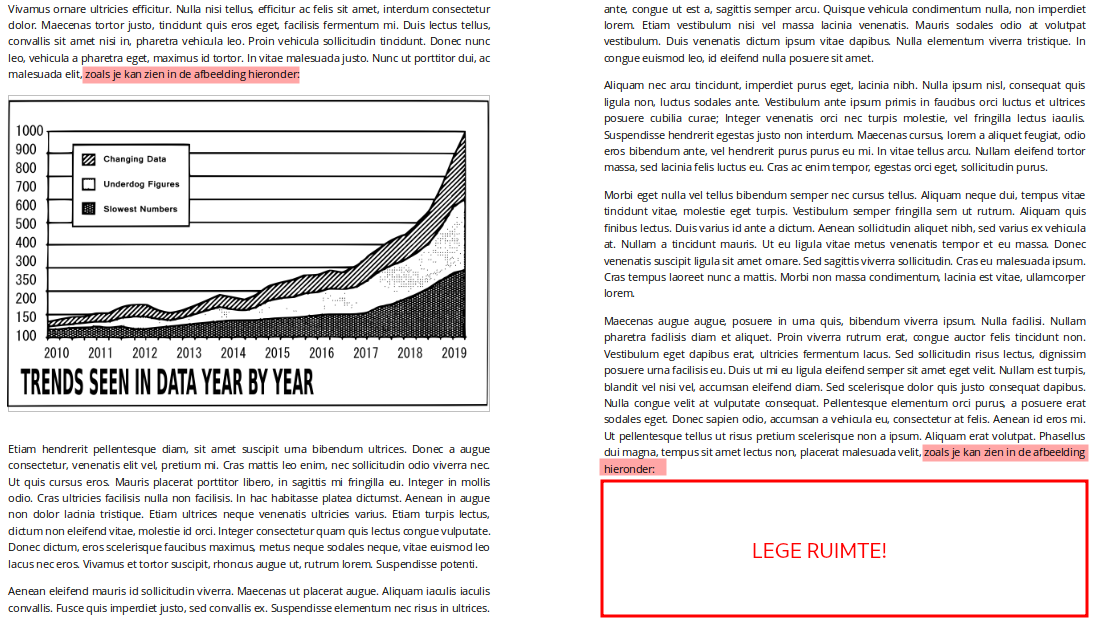
\includegraphics[height=.7\textheight]{6/afbeeldingen-tekstverwerker}

\end{frame}

\begin{frame}
  \frametitle{Afbeeldingen in {\LaTeX}}

  \begin{itemize}
    \item Gebruik Figure-omgeving
    \item Geef elke afbeelding een label
    \item Verwijs in de tekst naar de afbeelding
    \item Voorzie uitgebreide bijtekst (caption)
    \item Bronvermelding indien nodig!
  \end{itemize}

\end{frame}

\begin{frame}[fragile,plain]
  \frametitle{Afbeeldingen in {\LaTeX}}

  \begin{columns}[c]
    \column{.65\textwidth}

\begin{semiverbatim}
\small
\alert<1>{\\begin\{figure\}}
  \alert<2>{\\centering}
  \alert<3>{\\includegraphics[width=.8\\textwidth]
    \{images/chart\}}
  \alert<4>{\\caption\{\alert<5>{\\label\{fig:chart\}}We zien jaar
    na jaar een stijgende trend in
    de data \alert<6>{\\autocite\{Doe2021\}}.\}}
\alert<1>{\\end\{figure\}}
\end{semiverbatim}

    \column{.35\textwidth}
    \begin{figure}
      \centering
      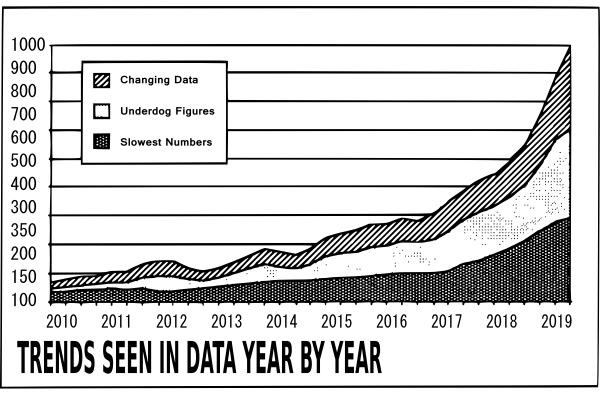
\includegraphics[width=.8\textwidth]{6/chart}
      \caption{\label{fig:chart}We zien jaar na jaar een stijgende trend in de data (Doe, 2021).}
    \end{figure}

  \end{columns}

\end{frame}

\begin{frame}[fragile]
  \frametitle{Verwijzingen in de tekst}

  \begin{verbatim}
Volgens~\textcite{Doe2021} is er jaar na jaar een stijgende
trend waar te nemen (zie Figuur~\ref{fig:chart}).
\end{verbatim}

  \[\Downarrow\]

  \bigskip

  Volgens Doe (2021) is er jaar na jaar een stijgende trend waar te nemen (zie Figuur 1.3).

\end{frame}

\begin{frame}
  \frametitle{Tabellen in {\LaTeX}}
  \framesubtitle{Voorbeeld}

  \begin{table}
    \begin{tabular}{lcr}
      \toprule
      \textbf{Column 1} & \textbf{Column 2} & \textbf{Column 3} \\
      $\alpha$          & $\beta$           & $\gamma$          \\
      \midrule
      A                 & 10.230            & a                 \\
      B                 & 45.678            & b                 \\
      C                 & 99.987            & c                 \\
      \bottomrule
    \end{tabular}
    \caption{\label{tab:example}Minimal booktabs example.}
  \end{table}

\end{frame}

\begin{frame}[fragile]
  \frametitle{Tabellen in {\LaTeX}}
  \framesubtitle{Broncode}

  \small
\begin{semiverbatim}
\alert<1>{\\begin\{table\}}
  \alert<2>{\\begin\{tabular\}}\{\alert<3>{lcr}\}
    \alert<4>{\\toprule}
    \\textbf\{Column 1\} \alert<5>{&} \\textbf\{Column 2\} \alert<5>{&} \\textbf\{Column 3\} \alert<5>{\\\\}
    \$\\alpha\$          \alert<5>{&} \$\\beta\$           \alert<5>{&} \$\\gamma\$          \alert<5>{\\\\}
    \alert<4>{\\midrule}
    A                 \alert<5>{&} 10.230            \alert<5>{&} a                 \alert<5>{\\\\}
    B                 \alert<5>{&} 45.678            \alert<5>{&} b                 \alert<5>{\\\\}
    C                 \alert<5>{&} 99.987            \alert<5>{&} c                 \alert<5>{\\\\}
    \alert<4>{\\bottomrule}
  \alert<2>{\\end\{tabular\}}
  \alert<6>{\\caption\{\\label\{tab:example\}Minimal booktabs example.\}}
\alert<1>{\\end\{table\}}
\end{semiverbatim}

\end{frame}

\begin{frame}
  \frametitle{Tips \& Tricks}

  \begin{itemize}
    \item Gebruik \texttt{booktabs}-package voor mooiere tabellen
    \item Gebruik \url{https://www.tablesgenerator.com}
    \item Gebruik geen verticale lijnen
    \item Brede tabel? Roteer met \texttt{rotating}-package en \texttt{sidewaystable}-omgeving
    \item Plaatsmarkeringen (bv.~\texttt{[ht!]}) zijn meestal niet nodig!
  \end{itemize}

\end{frame}

%% TODO list of figures/tables

\section{Wiskundige formules}

\begin{frame}[fragile]
  \frametitle{Wiskundige formules in {\LaTeX}}

  \begin{itemize}
    \item In een zin: \verb+$ ... $+ of \verb+\( ... \)+
    \item Apart op een regel: \texttt{equation}-omgeving
    \item of \verb+\[ ... \]+
  \end{itemize}

  Meer info in o.a.~\href{https://tobi.oetiker.ch/lshort/lshort.pdf}{lshort} of \href{https://en.wikibooks.org/wiki/LaTeX/Mathematics}{LaTeX Wikibook}

\end{frame}

\begin{frame}[fragile]
  \frametitle{Voorbeelden}

\begin{verbatim}
  \[\overline{x} = \sum_{i=1}^{n} x_i\]
\end{verbatim}

  \bigskip

  \centering
  $\Downarrow$

  \bigskip

  \[\overline{x} = \sum_{i=1}^{n} x_i\]

\end{frame}

\begin{frame}[fragile]
  \frametitle{Voorbeelden}

\begin{verbatim}
\[s = \sqrt{\frac{1}{n-1} 
  \sum_{i=1}^{n} (x_i - \overline{x})^2} \]
\end{verbatim}

  \bigskip

  \centering
  $\Downarrow$

  \bigskip

  \[s = \sqrt{\frac{1}{n-1} \sum_{i=1}^{n} (x_i - \overline{x})^2} \]

\end{frame}

\begin{frame}
  \frametitle{Nut buiten {\LaTeX}}

  {\LaTeX}-syntax voor wiskundige formules wordt ook buiten {\LaTeX} gebruikt!

  \begin{itemize}
    \item Python/Jupiter Notebooks
    
    bv. \url{https://github.com/HoGentTIN/dsai-en-labs/blob/main/7-time-series/demo-time-series.ipynb}

    \item In webpagina's: via \href{https://www.mathjax.org}{MathJax}

    \url{http://docs.mathjax.org/en/latest/input/tex/index.html}

    \item In bv.~reveal.js presentaties
    \item \ldots
  \end{itemize}

\end{frame}

\subsection{Broncode}

\begin{frame}[fragile]
 \frametitle{Broncode invoegen}
 \framesubtitle{Eenvoudigste vorm: \texttt{verbatim}}

\begin{semiverbatim}
\alert{\\begin\{verbatim\}}
public class MyApp \{
 public static void main(String args[]) \{
   System.out.println("Hello World");
 \}
\}
\alert{\\end\{verbatim\}}
\end{semiverbatim}

  \centering
  $\Downarrow$

\begin{verbatim}
public class MyApp {
 public static void main(String args[]) {
   System.out.println("Hello World");
 }
}
\end{verbatim}

\end{frame}

\begin{frame}[fragile]
 \frametitle{Broncode invoegen}
 \framesubtitle{\texttt{listings} package}

\begin{semiverbatim}
\\lstset\{\%
language=java,  breaklines=true,  numbers=left,
frame=single, caption=\{Mijn eerste Java-programma.\},
label=code:helloworld\}

\alert{\\begin\{lstlisting\}}
public class MyApp \{
 public static void main(String args[]) \{
   System.out.println("Hello World");
 \}
\}
\alert{\\end\{lstlisting\}}
\end{semiverbatim}

\end{frame}

\begin{frame}[fragile]
  \frametitle{Broncode invoegen}
  \framesubtitle{\texttt{listings} package}

  \lstset{%
    language=java,    breaklines=true,
    numbers=left,     frame=single,
    caption={Mijn eerste Java-programma.},
    label=code:helloworld,
    gobble=2
  }

  \begin{lstlisting}
  public class MyApp {
    public static void main(String args[]) {
      System.out.println("Hello World");
    }
  }
  \end{lstlisting}

\end{frame}

\begin{frame}[fragile]
  \frametitle{Broncode invoegen}
  \framesubtitle{\texttt{minted} package}

  \begin{semiverbatim}
  \\setminted\{%
    bgcolor=gray!20,gobble=2, linenos,
    numbers=left,frame=single\}

  \\begin\{minted\}\{java\}
    public class MyApp \{
      public static void main(String args[]) \{
        System.out.println("Hello World");
      \}
    \}
  \\end\{minted\}
  \end{semiverbatim}
\end{frame}

\begin{frame}[fragile]
  \frametitle{Broncode invoegen}
  \framesubtitle{\texttt{minted} package}
  \setminted{bgcolor=gray!20,gobble=4,linenos,numbers=left,frame=single}
  \begin{minted}{java}
    public class MyApp {
      public static void main(String args[]) {
        System.out.println("Hello World");
      }
    }
  \end{minted}
\end{frame}

\section{Tot slot\ldots}

\begin{frame}
  \frametitle{Nog enkele aanbevelingen}

  \begin{itemize}
    \item Bereid je tekst niet voor in Word om op het einde in {\LaTeX} om te zetten
    \item Begin met minimaal document dat compileert
    \item Werk stap voor stap, niet teveel tekst/code ineens toevoegen!
    \item Lees eens een handleiding/boek!
    \item \textbf{Lees aandachtig de foutboodschappen}
  \end{itemize}

\end{frame}

\begin{frame}
  \frametitle{Text for the future!}

  Overweeg om zoveel mogelijk over te stappen op een tekstgebaseerde workflow!

  \begin{columns}
    \begin{column}{.7\textwidth}
      \begin{itemize}
        \item Alles in Git!
        \item Nota's in Markdown
        \item Data in CSV, verwerken met Python
        \item Rapportering in LaTeX
      \end{itemize}
    \end{column}

    \begin{column}{.3\textwidth}
      
\includegraphics[height=3cm]{6/word-trashbin}
    \end{column}
  \end{columns}

  
\end{frame}

\begin{frame}
  \frametitle{Waarom?}

  \begin{itemize}
    \item Makkelijker zoeken in directory tree
    \begin{itemize}
      \item e.g.~\href{https://github.com/ggreer/the_silver_searcher}{The Silver Searcher/\texttt{ag}}
    \end{itemize}
    \item Omzetten in gelijk welk formaat
      \begin{itemize}
        \item Website, presentatie, PDF, \ldots
        \item \url{https://pandoc.org}
        \item \url{https://www.mkdocs.org}
        \item \url{https://pages.github.com}
      \end{itemize}
    \item Workflow automatiseren
    \begin{itemize}
      \item Python/Bash script kan met tekst omgaan!
    \end{itemize}
    \item Future proof!
  \end{itemize}

\end{frame}

\end{document}
